\section{Editor Design}
\label{sec:editor_design}
Programming the cell is an essential part of the game. This is where the user will learn basic constructs in the imperative paradigm by using them to program the cells.

The editor is used by the player to design their program, that will be executed during the game. To keep the overall game experience consistent, the editor will be using the same hexagonal design as the playing field. The programming will be done visually, and the hexagonal design will give the user more options for organizing their program.\\

The editor consists of two main parts, the programming grid of hexagons on the left, and individual customization of instructions on the right. An illustration can be seen on \autoref{fig:editor}.

\begin{figure}[ht]
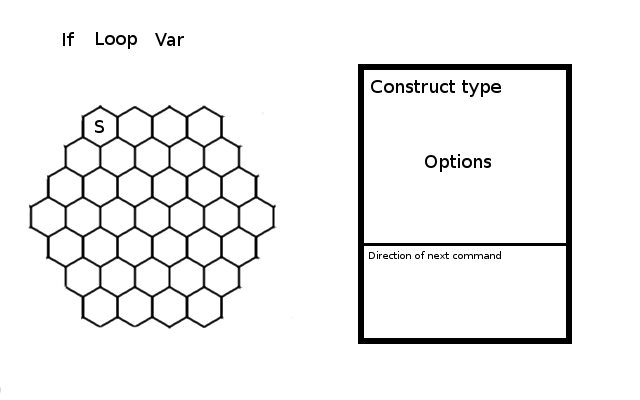
\includegraphics[width=\textwidth]{img/editor.png}
\caption{Preliminary design of the editor.}
\label{fig:editor}
\end{figure}

\subsubsection*{Programming Grid}
The programming grid makes use of an interface, similar to that of the game 'Carnage Heart' but with drag-and-drop.
Each programming construct, e.g. if-statements and loops, can be dragged from the top of the screen onto the hexagonal grid.
Initially this hexagonal grid only has a start point, and it is up to the player to create the program.
The program will be running from the start point on the grid.

It should be noted, that programming the cell should not be the cause of frustration due to the occurrence of peculiar programming-oriented errors, which the player will have to deal with.
For this reason, it is important that the interface does not give the user the chance to make fatal errors such as type errors.\newline

Since the editor is using a drag-and-drop interface, adding new functionality to a program is done by dragging a construct onto the grid, and customizing it.
Since the aim of the game is to teach programming without doing so explicitly, the variables can be define as three types.
These are: numbers, entities, and directions.
The idea is that by limiting variables to three categories with meaningful names, the player will hopefully be able to easily understand what happens without prior knowledge to types in programming.

\subsubsection*{Instruction Customization}
The instruction customization is activated, when the player clicks on a construct, that has been placed on the hexagonal grid.
If it is deselected the instruction customization disappears until another construct is selected.
It will show different information depending on what kind of construct the player has clicked on.
For example, for the if-statement it should to be possible to choose what to compare and the comparison type (equal, not equal etc).
The bottom part of the instruction customization is used by the player to choose, which tile on the hexagonal grid the program should be going to next.
This can be used to structure the program or make it possible for the player to customize the grid to their liking.
However, it also allows the user the freedom to create infinite loops.
Since this is the Halting Problem and its solution does not exist, we can not check the program for infinite loops for the user.
Therefore, we leave it up to the user to find these loops. 